% CHAPTER_BEGIN
\section{Arch Framework: Research Report}

\subsection{Introduction}

The \textit{arch} project represents a custom made framework for writing mainly HPC data applications. Is built as a framework on top of IPL (Ibis Portability Layer - communication layer) adopting a master-slave architecture. The master is basically another slave that hast the extra task to setup the communication and start splitting the job between all the nodes (slaves). Thus, we do not have to install and configure anything as an independent platform and then use a special API to run jobs/tasks on top of that platform (i.e such as using Hadoop). With other words, what we need to run an \textit{arch} application is the \textit{ibis-server} (it is embedded inside the \textit{arch} framework so we can run it from there and have our inter nodes communication layer) and, of course, a program that uses \textit{arch} to compute some data. Usually, the program does not have to be divided into a master and slave side. We can use \textit{arch} framework only to write the master section. The slaves' behavior is automatically dictated by the list of actions that we add in the code, inside the job. For testing my experimental changes on \textit{arch} I have run \textit{querypie:BenchmarkSorting}, an application built with \textit{arch} framework that sorts large data-sets of RDF triples. To build and run this entire setup (\textit{arch} + \textit{querypie}) I have used the git repository for code deployment on DAS4 and a self written ant file \cite{build_file} to build \textit{querypie} into a .jar bundle package (a package that embeds inside all the necessary dependencies, including the \textit{arch.jar} package built with the default ant file). Next, to run the \textit{querypie} on DAS4 was a simple \textit{prun} command execution (see next section).

% 
\subsection{Deployment \& execution on DAS4}

For \textit{arch} and \textit{querypie} main-code deployment on DAS4 you will first need access to their git repositories \cite{arch_repo}, \cite{qpie_repo}. After that, simply clone their repositories in your home DAS4 directory and be sure that you are located in the benchm\_master branch. For the entire list of steps that you have to follow in order to run/execute this setup on multiple nodes, read next.
\newline
\newline
\textbf{Steps for running \textit{querypie} on multiple DAS4 cluster nodes:}
\begin{enumerate}
	\item Deploy \textit{arch} and \textit{querypie} projects in your home DAS4 directory. Each project already has all the dependencies packages and ant files necessary for automatic build. 
	\item Build \textit{arch} project using its ant build file: 'ant build-jar' 
	\item Copy the \textit{arch.jar} package in the \textit{/lib} directory of the \textit{querypie}
	\item Build \textit{querypie} project using its ant build file \cite{build_file}: 'ant build-jar' (will create a .jar bundle package that we use to execute its main class - BenchmarkSorting - on DAS4; the .jar is placed by default in the \textit{/jar} directory -- for any change you wish to do look for the parameters inside the ant file)
	\item Configure \textit{ibis-server} parameters (port, enable events, etc) from inside \textit{arch's} ant build file 
	\item Start \textit{ibis-server} on the DAS4 head-node from the \textit{arch} project directory: 'ant ibis-server' (note the address and port that is using)
	\item Run/execute \textit{querypie} on DAS4 using the script example \cite{run_on_das4} -- change the parameters for your own needs.
\end{enumerate}

% 
\subsection{Workflow example: how \textit{arch} can be used to sort RDF triples}

In this section I will explain how the \textit{arch} framework works on 'crunching' data, using as a workflow example the RDF triples' \textit{distributed sorting} implemented in \textit{querypie}, BenchmarkSorting. To begin with, the process of sorting can be split in 3 steps: (1) read and sort the RDF triples; (2) send-receive communication; (3) merge and write the RDF triples in files;

The main data structure used in all three steps is the 'Bucket' -- an in-memory buffer that is filled up with triples of which hash keys are equal to the bucket's identifier. When the buffer limit size is exceeded, all its content gets sorted and cached on the hard-disk (in files). Thus, when we refer to the 'Bucket' we usually mean both the in-memory buffer and the hard-disk stored files (if data hits the disk). Each time the files' number increases above a fixed limit, a thread is started to merge them 2-by-2 up until their number gets below. All the information about the files (metadata such as names, first elements, size, etc) is kept inside the Bucket -- we need them at the time we transfer the triples or when we write the resulted set back. By default, each node keeps 1 bucket in the memory for every other node (remote-buckets), including itself (local-bucket). So, there are by default N buckets on each node, where N = number of nodes; a new feature allows you to use more than 1 bucket per node (NPARTITIONS\_PER\_NODE parameter, which by default is 1). The creation and initialization of a bucket (create, get, release, etc) is controlled by the 'Buckets' wrapper class.

% 
\subsubsection*{(1) Read and sort the RDF triples}

First, the data set (compressed or not) gets split in file partitions of almost the same sizes, each one being assigned to one node for further reading. The split of the data set is done by the ReadFromFiles action, which creates FileCollections of a 'minimumFileSplitSize'. Next, the FileLayer of each node reads the triples from its assigned partitions -- the FileCollections (a set of pathnames representing the partitioned files) -- and inserts them into the corresponding local/remote bucket (where the triple's hash key equals to the node's bucket id). If a bucket gets full with triples, its content is sorted using the java MergeSort algorithm and cached on disk. All the information/metadata about caching that content on the disk is stored inside the Bucket object for further use. When there is no more data left to read from a partition, the node broadcasts a signal alert that the remote-buckets are ready to get transferred (this means that the send-receive start is dependent on the size of the file partition). So, at this point, the send-receive step begins -- triples are transferred from the remote-buckets to their assigned nodes (i.e. on node Y, its remote-bucket for node X has triples assigned to X \textit{=>} triples from Y's remote-bucket will be transferred to X's local-bucket).

\begin{figure}
\centering
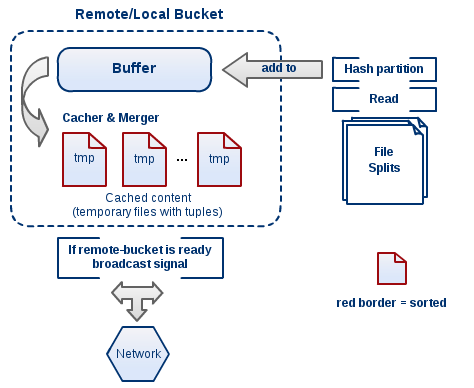
\includegraphics[scale=0.6]{diag1}
\caption{Read and sort - remote \& local buckets structure}
\end{figure}

% 
\subsubsection*{(2) Send-receive communication}

When a signal alert for a bucket ready for transfer is received by a node (\textit{receiver}), a corespondent request for fetching triples from it is sent back to the \textit{sender}. Then, the \textit{sender} registers that request and, whenever the remote-bucket has the available data (MIN\_SIZE\_TO\_SEND) for transfer, removes a chunk and sends it to the \textit{requester}. Next, the \textit{recipient} adds that chunk into its local-bucket and \textit{sends} a request for another fetch. As long as on the other side (\textit{sender's} side) the remote-bucket still contains triples, the \textit{receiver} will have chunks get transferred in its local-bucket. If there are no more RDF triples inside of it, the remote-bucket is released and the transfer's metatada are cleaned/removed. But, before that, a last signal that marks the end of the transfer is sent to the \textit{recipient}, which flags its local-bucket with \textit{finished} -- meaning that is ready for merge \& write. The chunk removal, in the worst case when triples are getting cached on the disk, has to extract all the minimum triples from the in-memory buffer and the cached files (in sorted order) up until it fills the chunk. Is necessary to do that because we expect to receive sorted data on the \textit{recipient} side. Otherwise, basically, it sends a chunk directly from the in-memory buffer, but after it applies the sort.

\begin{figure}
\centering
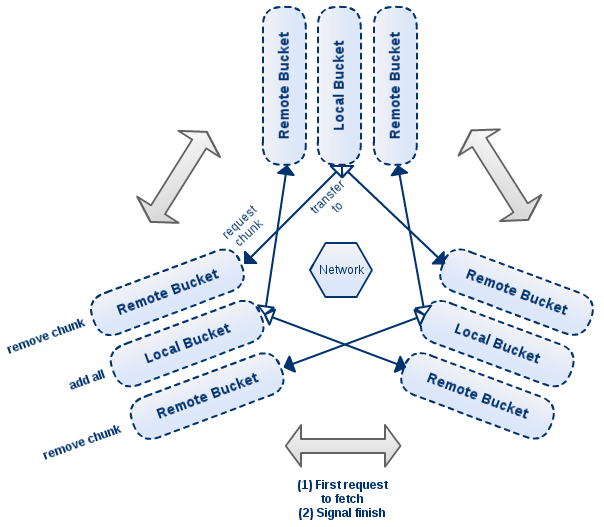
\includegraphics[scale=0.6]{diag2}
\caption{Transfer to correspondent nodes - send-receive communication}
\end{figure}

% 
\subsubsection*{(3) Merge and write the RDF triples in files - results output}

After all the triples got moved from the remote-buckets (previous step is finished), the final step is all about merging the local-bucket's in-memory buffer with its cached content (the files from the hard disk) -- in case data hits the disk. This task is done by the same method (RemoveChunk) that removes chunks for triples' transfer. Now it stands for fetching data from the local-bucket whenever the bucket-iterator is called for writing data. In the end, the result at each node is represented by one sorted file with RDF triples (only if we let the default number, equal with 1, of buckets per node). 

\begin{figure}
\centering
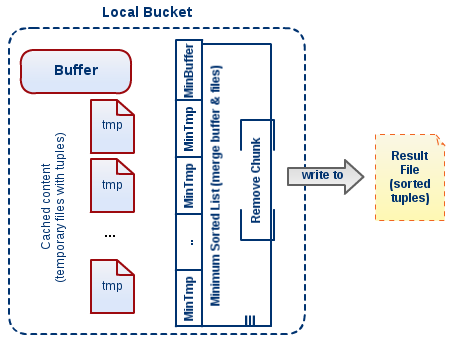
\includegraphics[scale=0.6]{diag3}
\caption{Merge and write}
\end{figure}

\pagebreak

% 
\subsection{Execution-time \& profiling}

<Table-1>
<Chart-1>

% 
\subsubsection*{Discussion}

% 
\subsection{Proposals \& implementations: how to improve \textit{arch's} \\ execution-time}

In generally, a distributed large scale data application is considered optimal if each data-item (in our case \textit{1 single RDF triple}) is processed (i.e \textit{distributed sorting}) using less than 2 writes on disk. Not so many applications apply this rule - including the Arch framework (branch benchm\_master). In worst case, if we are dealing with a big amount of data (a file partition split size bigger than the amount of memory - buffer size - available on each node), the total number of disk writes sums up to 3 (1 write would for reading-sorting-caching data on the disk + 1 on the recipient side for gathering data in the local-bucket and + 1 for writing the final results). Given the pre-research I made on Hadoop:Map-Reduce \cite{hadoop}, a platform for processing data which has a stage called 'shuffle' \cite{shuffling} that ensures data is partitioned and sent to the reducers, I came up with the following ideas: 
\begin{itemize}
\item to \textit{disable the local sorting of remote-buckets},
\item to \textit{start as soon as possible the triples' transfer/send-receive} (we do not need to keep data more than is necessary => until the end of a partition read) and
\item to \textit{'hide' the triples' merging} under a independent background process. 
\end{itemize}
  
These proposals intent to increase the chances of using less then 3 writes on disk (unless the network represents a bottleneck) and to improve the execution time of the Arch framework. From the distributed-sorting point of view, in my opinion, this approach of moving the sort phase on the recipient side and having less writes on disks is able to improve the total time of the execution. In the next paragraphs I will detail each of them, writing also about the implementation aspects.

% 
\subsubsection*{(1) Disabling sort property for remote-buckets}

Now, that we decided to begin the data transfer as soon as possible, we do not need anymore to apply a sorting algorithm on the remote-buckets before that (sooner we send the chunks into network, lower the chances to hit the disk would be). The sorting will have to be placed on the recipient side (local-bucket), under the same assumptions -- when the buffer gets filled, it gets sorted and cached on the disk. To disable this property, we have to construct/initialize the remote-buckets without a sorting function and sorting parameters.

% 
\subsubsection*{(2) Interleave the transfer with the local reading}

For the transfer to start at the very beginning is obvious that it should be overlap the files-partition read step (triples' reading). So, in startTransfer() we should start broadcasting signal alerts to the other nodes for sending back requests for bucket fetch -- alertTransfer() method. To allow that, few changes have to be done:

\textbf{(a) Allow receiving of unsorted data}

When a chunk is getting transferred (\textit{sendTuples() method}) we specify the sorting function and its parameters in the message. Because we do not apply anymore a sorting algorithm on the remote-buckets we now declare a null sorting function and parameters (meaning that the chunk is not sorted). Thus, on the recipient side we have to allow appending of unsorted data into the local-bucket. The original version of \textit{addAll()} method, which adds chunks into the local-bucket, used to expect sorted data -- it compares the size of the chunk with the size of the buffer and depending on which is bigger that one is being cached on the disk (\textit{cacheBuffer() method}). If it happens that the chunk is bigger, is cached directly without being sorted (because it was already done that on the sender side), otherwise it sorts the buffer and spills it on the disk. For the research part, this logic got changed a bit -- we now first try to add the chunk into the buffer, or the other way if the buffer has fewer elements, instead of writing directly onto the disk. Only if the addition fails, we sort and cache in a temporary file the one's content that has a bigger size.

\textbf{(b) Split the main buffer into two buffers}

Furthermore, we can improve the previous part by splitting the main buffer into two separate buffers in such way that one should be use for reading (\textit{inBuffer}) and one for receiving chunks (\textit{exBuffer}). In this way, we can operate independently on each buffer. One disadvantage is that we require extra memory for the second buffer. At the end of the transfer -- when the bucket is flagged with finished -- we add one buffer into another (\textit{combineInExBuffers()} method) in order to have a single buffer combined with both contents. If both have big sizes, one of them (the smaller one) gets cached on the disk.

\textbf{(c) Loosen-up the synchronization between bucket's methods}

Now, that we split the buffer into two independent buffers we can further loosen-up the synchronization primitives between the read and transfer (\textit{add() and addAll() methods}), the only coarse synchronization point being the moment when both methods call \textit{cacheBuffer()} (both buffers might get full maybe at the same time).

\begin{figure}
\centering
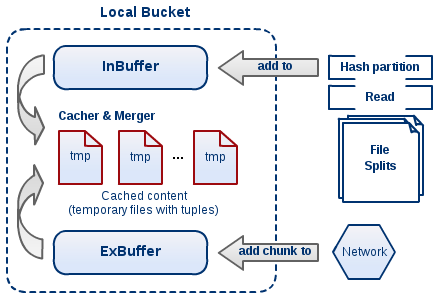
\includegraphics[scale=0.6]{diag4a}
\linebreak
\linebreak
\centering
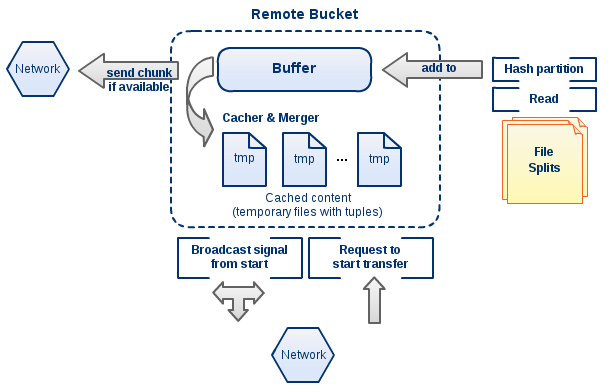
\includegraphics[scale=0.6]{diag4b}
\caption{New local/remote buckets}
\end{figure}

% 
\subsubsection*{(3) In-background chunks' removal for writing the results in files}

The last idea refers to the writing of the sorted local-bucket (all the triples) into the result file -- the result set. The way of doing that is to use the \textit{removeChunk()} method into the \textit{bucketIterator} class to fetch chunks from the local-bucket when there are no more triples to iterate on. An idea would be to hide the dead-time that the iterator has to wait for merging-up triples from the main memory (buffer) with the ones stored on the disk and to try instead to remove/get a chunk that has been already processed and stored in a set of auxiliary buffers in memory (triples ready to be written as results). For that, we start a separate thread at the right moment we set the bucket's flag on finished, which fills up auxiliary buffers with chunks from the main buffer. When a write is being performed (iterator is called), the chunk is taken directly from the auxiliary buffers instead of waiting for the whole merge. Moreover, when a buffer from the set gets emptied the thread will go on and try to refill it, if there are anymore elements for that -- this mechanism of storing buffers processed earlier is generally called 'Double-Buffering'.

\begin{figure}
\centering
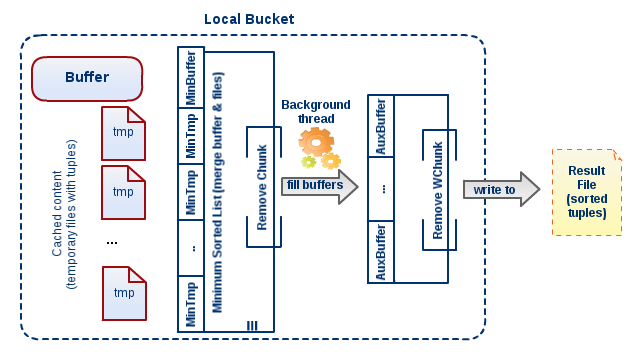
\includegraphics[scale=0.6]{diag5}
\caption{In-background merge-up}
\end{figure}

% 
\subsubsection{Results: execution-time \& profiling}

<Table-2>
<Chart-2>

% 
\subsubsection*{Discussion}

\subsection{Future work}

\subsection{Conclusions}
% CHAPTER_END